\chapter{Code Snippets}
\label{chap:code_snippets}

% PyTorch neural network defining the DQN model layers and forward pass
\section{DQN Network Architecture}
\label{sec:dqn_architecture}
The following snippet defines the architecture of the \gls{dqn} model used for traffic signal control.

\begin{lstlisting}[language=Python, caption={DQN Model Architecture}]
import torch
import torch.nn as nn

class DQNetwork(nn.Module):

    def __init__(self, state_size, action_size):
        super(DQNetwork, self).__init__()
        self.fc1 = nn.Linear(state_size, 128)
        self.fc2 = nn.Linear(128, 64)
        self.fc3 = nn.Linear(64, action_size)
        
    def forward(self, x):
        x = torch.relu(self.fc1(x))
        x = torch.relu(self.fc2(x))
        x = self.fc3(x)
        return x
\end{lstlisting}

% Circular buffer for storing and sampling experience tuples during training
\section{Replay Buffer}
\label{sec:replay_buffer}
This snippet demonstrates how experiences (state, action, reward, next state, done) are stored and sampled in the replay buffer.

\begin{lstlisting}[language=Python, caption={Replay Buffer Implementation}]
from collections import deque
import random
import numpy as np

class ReplayBuffer:

    def __init__(self, buffer_size):
        self.buffer = deque(maxlen=buffer_size)
    
    def add(self, state, action, reward, next_state, done):
        self.buffer.append((state, action, reward, next_state, done))

    
    def sample(self, batch_size):
        batch = random.sample(self.buffer, batch_size)
        states, actions, rewards, next_states, dones = zip(*batch)
        return (
            np.array(states),
            np.array(actions),
            np.array(rewards),
            np.array(next_states),
            np.array(dones)
        )


        
    
    def size(self):
        return len(self.buffer)
\end{lstlisting}

% Agent class handling action selection, exploration policy, and network management
\section{DQN Agent}
\label{sec:dqn_agent_code}
This snippet defines the \gls{dqn} agent that interacts with the traffic control environment, selecting actions and updating the model.

\begin{lstlisting}[language=Python, caption={DQN Agent Implementation}]
import torch.optim as optim

class DQNAgent:

    def __init__(self, state_size, action_size):
        self.state_size = state_size
        self.action_size = action_size
        self.gamma = 0.99
        self.epsilon = 1.0
        self.epsilon_min = 0.1
        self.epsilon_decay = 0.995
        self.learning_rate = 0.001
        self.batch_size = 32
        self.device = torch.device("cuda" if torch.cuda.is_available() else "cpu")
        self.q_network = DQNetwork(state_size, action_size).to(self.device)
        self.target_network = DQNetwork(state_size, action_size).to(self.device)
        self.update_target_network()
        self.optimizer = optim.Adam(self.q_network.parameters(), lr=self.learning_rate)
        self.replay_buffer = ReplayBuffer(10000)
        self.criterion = nn.MSELoss()
    
    def update_target_network(self):
        self.target_network.load_state_dict(self.q_network.state_dict())
    
    def act(self, state, training=True):
        if training and random.random() < self.epsilon:
            return random.randrange(self.action_size)
        
        with torch.no_grad():
            state_tensor = torch.FloatTensor(state).unsqueeze(0).to(self.device)
            q_values = self.q_network(state_tensor)
            return q_values.argmax().item()
\end{lstlisting}

% Training loop performing experience replay, loss computation, and weight updates
\section{Model Training}
\label{sec:model_training_code}
This snippet demonstrates the process of training the \gls{dqn} agent, including experience replay and the loss calculation.

\begin{lstlisting}[language=Python, caption={Training the DQN Agent}]
    def replay(self):
        if self.replay_buffer.size() < self.batch_size:
            return 0.0 

        states, actions, rewards, next_states, dones = self.replay_buffer.sample(self.batch_size)
        states = torch.FloatTensor(states).to(self.device)
        actions = torch.LongTensor(actions).to(self.device)
        rewards = torch.FloatTensor(rewards).to(self.device)
        next_states = torch.FloatTensor(next_states).to(self.device)
        dones = torch.FloatTensor(dones).to(self.device)

        current_q_values = self.q_network(states).gather(1, actions.unsqueeze(1)).squeeze(1)
        
        with torch.no_grad():
            next_q_values = self.target_network(next_states).max(1)[0]
            target_q_values = rewards + (1 - dones) * self.gamma * next_q_values
        
        loss = self.criterion(current_q_values, target_q_values)

        self.optimizer.zero_grad()
        loss.backward()
        self.optimizer.step()
        
        return loss.item()
\end{lstlisting}

% Functions for persisting and restoring the trained model state to and from disk
\section{Model Saving and Loading}
\label{sec:model_io}
The following snippet shows how to save and load the model state.

\begin{lstlisting}[language=Python, caption={Model Saving and Loading}]
    def save(self, filepath):
        torch.save({
            'q_network_state_dict': self.q_network.state_dict(),
            'target_network_state_dict': self.target_network.state_dict(),
            'optimizer_state_dict': self.optimizer.state_dict(),
            'epsilon': self.epsilon
        }, filepath)
        print(f"Model saved to {filepath}")
    
    def load(self, filepath):
        checkpoint = torch.load(filepath)
        self.q_network.load_state_dict(checkpoint['q_network_state_dict'])
        self.target_network.load_state_dict(checkpoint['target_network_state_dict'])
        self.optimizer.load_state_dict(checkpoint['optimizer_state_dict'])
        self.epsilon = checkpoint['epsilon']
        print(f"Model loaded from {filepath}")
\end{lstlisting}

% Brief recap of the code appendix and its purpose
\section{Summary}
\label{sec:code_summary}
The presented code snippets demonstrate the practical implementation of the \gls{dqn}-based traffic control system. These snippets highlight how reinforcement learning and neural networks are applied to optimize traffic flow at the Thapathali intersection.

\chapter{Project Budget}
\label{chap:project_budget}

% Breakdown of estimated project costs and resource allocation
This project is designed to be completed with minimal cost by relying on open-source tools (\eg \gls{sumo}) and free software resources. The \gls{dqn} development and training will be performed using available local computing resources. If additional compute is needed, we will use free-tier subscriptions, academic/free credits (if available), or support from friends/peers with suitable hardware instead of paid cloud services. Therefore, the budget mainly covers documentation and small miscellaneous expenses.

\begin{table}[H]
    \centering
    \small
    \caption{Project Budget Allocation}
    \label{tab:budget_allocation}
    \begin{tabular}{p{7cm}p{3cm}c}
        \toprule
        \textbf{Task} & \textbf{Cost (NRP)} & \textbf{Total (NRP)} \\
        \midrule
        Documentation (printing, binding, stationery) & RS. 1200 & RS. 1200 \\
        Miscellaneous & RS. 1000 & RS. 1000 \\
        \midrule
        \multicolumn{2}{r}{\textbf{Total}} & \textbf{RS. 2200} \\
        \bottomrule
    \end{tabular}
\end{table}

\chapter{Project Timeline}
\label{chap:project_timeline}

% Gantt chart illustrating phased milestones and deliverable schedule
The project will be organized into distinct phases, each focusing on specific tasks with well-defined milestones. These phases will ensure structured and efficient progress, with regular evaluations to monitor the advancement toward successful project completion.

\section{Gantt Chart}
\label{sec:gantt_chart}

\begin{figure}[H]
    \centering
    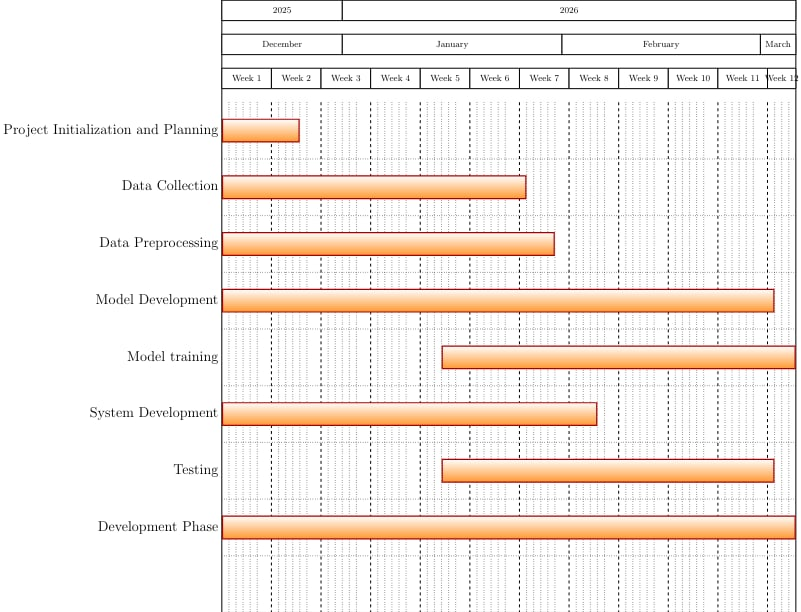
\includegraphics[width=\textwidth]{src/images/figures/gantt_chart.jpeg}
    \caption{Project Gantt Chart}
    \label{fig:gantt_chart_fig}
\end{figure}


\chapter{Summary of Data}
\label{chap:data_summary}

% Tabulated vehicle count and PCU origin-destination data used for simulation calibration
This dataset includes portions of vehicle counts alongside \gls{pcu} \gls{od} data:

\begin{table}[h!]
    \centering
    \small
    \caption{15-Minute Interval Vehicle Counts by Class: Day 1 (06:00--15:15)}
    \label{tab:time_data_part1}
    \begin{tabular}{ccccccccccccc}
        \toprule
        \textbf{Start Time} & \textbf{End Time} & \textbf{HV} & \textbf{LV} & \textbf{B} & \textbf{MB} & \textbf{MIB} & \textbf{C} & \textbf{U} & \textbf{F} & \textbf{T} & \textbf{TW} \\
        \midrule
        06:00:00 & 06:15:00 & 0 & 3 & 19 & 4 & 23 & 107 & 26 & 9 & 18 & 545 \\
        06:15:00 & 06:30:00 & 0 & 4 & 15 & 13 & 34 & 166 & 38 & 14 & 22 & 780 \\
        06:30:00 & 06:45:00 & 3 & 8 & 24 & 12 & 35 & 153 & 38 & 24 & 28 & 828 \\
        06:45:00 & 07:00:00 & 3 & 3 & 34 & 9 & 34 & 189 & 35 & 37 & 30 & 963 \\
        07:00:00 & 07:15:00 & 1 & 5 & 28 & 9 & 35 & 207 & 38 & 32 & 21 & 956 \\
        07:15:00 & 07:30:00 & 2 & 4 & 29 & 14 & 45 & 229 & 36 & 42 & 24 & 993 \\
        07:30:00 & 07:45:00 & 0 & 7 & 28 & 12 & 31 & 304 & 45 & 58 & 27 & 1093 \\
        07:45:00 & 08:00:00 & 4 & 4 & 32 & 9 & 39 & 270 & 38 & 48 & 26 & 1102 \\
        08:00:00 & 08:15:00 & 0 & 6 & 18 & 13 & 38 & 265 & 46 & 53 & 31 & 1048 \\
        08:15:00 & 08:30:00 & 2 & 7 & 34 & 7 & 33 & 324 & 34 & 58 & 26 & 1093 \\
        08:30:00 & 08:45:00 & 1 & 4 & 36 & 12 & 37 & 333 & 39 & 53 & 25 & 1137 \\
        08:45:00 & 09:00:00 & 1 & 5 & 27 & 7 & 44 & 368 & 43 & 66 & 29 & 1332 \\
        09:00:00 & 09:15:00 & 0 & 3 & 23 & 9 & 39 & 356 & 33 & 73 & 34 & 1434 \\
        09:15:00 & 09:30:00 & 2 & 6 & 21 & 14 & 33 & 376 & 27 & 84 & 35 & 1689 \\
        09:30:00 & 09:45:00 & 0 & 4 & 26 & 10 & 39 & 379 & 30 & 89 & 37 & 1957 \\
        09:45:00 & 10:00:00 & 0 & 3 & 20 & 10 & 40 & 383 & 21 & 78 & 45 & 2117 \\
        10:00:00 & 10:15:00 & 0 & 2 & 20 & 11 & 41 & 421 & 33 & 64 & 37 & 2155 \\
        10:15:00 & 10:30:00 & 0 & 5 & 18 & 13 & 41 & 448 & 33 & 87 & 40 & 2027 \\
        10:30:00 & 10:45:00 & 1 & 3 & 25 & 10 & 41 & 433 & 37 & 76 & 33 & 1824 \\
        10:45:00 & 11:00:00 & 0 & 6 & 21 & 15 & 37 & 445 & 51 & 90 & 33 & 1880 \\
        11:00:00 & 11:15:00 & 0 & 2 & 23 & 8 & 33 & 452 & 43 & 97 & 40 & 1904 \\
        11:15:00 & 11:30:00 & 1 & 6 & 24 & 4 & 39 & 461 & 47 & 95 & 29 & 1840 \\
        11:30:00 & 11:45:00 & 1 & 5 & 21 & 10 & 44 & 455 & 68 & 85 & 36 & 1921 \\
        11:45:00 & 12:00:00 & 1 & 4 & 22 & 9 & 39 & 454 & 64 & 94 & 33 & 1968 \\
        12:00:00 & 12:15:00 & 1 & 3 & 20 & 12 & 40 & 480 & 62 & 105 & 21 & 1970 \\
        12:15:00 & 12:30:00 & 0 & 4 & 24 & 8 & 33 & 435 & 59 & 88 & 26 & 1963 \\
        12:30:00 & 12:45:00 & 0 & 5 & 24 & 9 & 39 & 448 & 73 & 91 & 31 & 2025 \\
        12:45:00 & 13:00:00 & 1 & 3 & 23 & 8 & 34 & 442 & 66 & 107 & 32 & 1953 \\
        13:00:00 & 13:15:00 & 1 & 6 & 21 & 7 & 39 & 447 & 69 & 96 & 24 & 1817 \\
        13:15:00 & 13:30:00 & 1 & 6 & 22 & 10 & 36 & 507 & 69 & 117 & 27 & 1453 \\
        13:30:00 & 13:45:00 & 0 & 7 & 24 & 6 & 38 & 541 & 80 & 117 & 35 & 1289 \\
        13:45:00 & 14:00:00 & 1 & 5 & 24 & 10 & 34 & 471 & 57 & 104 & 24 & 1078 \\
        14:00:00 & 14:15:00 & 1 & 11 & 20 & 9 & 33 & 465 & 41 & 93 & 18 & 1176 \\
        14:15:00 & 14:30:00 & 1 & 7 & 16 & 8 & 36 & 506 & 50 & 112 & 26 & 1392 \\
        14:30:00 & 14:45:00 & 2 & 9 & 23 & 13 & 28 & 499 & 58 & 120 & 28 & 1595 \\
        14:45:00 & 15:00:00 & 0 & 4 & 22 & 6 & 36 & 507 & 65 & 106 & 27 & 1608 \\
        15:00:00 & 15:15:00 & 0 & 6 & 22 & 8 & 29 & 496 & 51 & 131 & 29 & 1647 \\
        \bottomrule
    \end{tabular}
\end{table}

\clearpage

\begin{table}[h!]
    \centering
    \small
    \caption{15-Minute Interval Vehicle Counts by Class: Day 1 (15:15--22:15)}
    \label{tab:time_data_part2}
    \begin{tabular}{ccccccccccccc}
        \toprule
        \textbf{Start Time} & \textbf{End Time} & \textbf{HV} & \textbf{LV} & \textbf{B} & \textbf{MB} & \textbf{MIB} & \textbf{C} & \textbf{U} & \textbf{F} & \textbf{T} & \textbf{TW} \\
        \midrule
        15:15:00 & 15:30:00 & 0 & 1 & 22 & 5 & 39 & 502 & 51 & 93 & 34 & 1572 \\
        15:30:00 & 15:45:00 & 0 & 9 & 20 & 7 & 37 & 478 & 49 & 102 & 26 & 1578 \\
        15:45:00 & 16:00:00 & 1 & 0 & 20 & 13 & 34 & 454 & 54 & 111 & 28 & 1485 \\
        16:00:00 & 16:15:00 & 0 & 5 & 21 & 12 & 34 & 455 & 41 & 107 & 25 & 1536 \\
        16:15:00 & 16:30:00 & 0 & 1 & 19 & 12 & 39 & 477 & 44 & 112 & 20 & 1576 \\
        16:30:00 & 16:45:00 & 1 & 4 & 22 & 8 & 36 & 494 & 45 & 108 & 37 & 1704 \\
        16:45:00 & 17:00:00 & 0 & 3 & 27 & 8 & 35 & 462 & 48 & 140 & 29 & 1621 \\
        17:00:00 & 17:15:00 & 0 & 8 & 17 & 9 & 41 & 442 & 33 & 121 & 22 & 1606 \\
        17:15:00 & 17:30:00 & 0 & 5 & 25 & 5 & 45 & 476 & 32 & 126 & 24 & 1735 \\
        17:30:00 & 17:45:00 & 0 & 2 & 17 & 12 & 37 & 459 & 34 & 122 & 25 & 1716 \\
        17:45:00 & 18:00:00 & 1 & 7 & 24 & 12 & 39 & 465 & 27 & 107 & 16 & 1735 \\
        18:00:00 & 18:15:00 & 0 & 5 & 17 & 8 & 34 & 415 & 30 & 99 & 19 & 1782 \\
        18:15:00 & 18:30:00 & 0 & 3 & 28 & 10 & 37 & 430 & 39 & 108 & 20 & 1698 \\
        18:30:00 & 18:45:00 & 0 & 8 & 18 & 8 & 36 & 372 & 23 & 139 & 14 & 1462 \\
        18:45:00 & 19:00:00 & 0 & 5 & 13 & 8 & 32 & 363 & 35 & 105 & 16 & 1327 \\
        19:00:00 & 19:15:00 & 2 & 6 & 25 & 9 & 29 & 331 & 30 & 100 & 12 & 1347 \\
        19:15:00 & 19:30:00 & 1 & 10 & 13 & 4 & 26 & 348 & 31 & 88 & 8 & 1368 \\
        19:30:00 & 19:45:00 & 1 & 4 & 13 & 2 & 30 & 353 & 33 & 90 & 4 & 1309 \\
        19:45:00 & 20:00:00 & 1 & 5 & 5 & 0 & 20 & 339 & 30 & 82 & 5 & 1152 \\
        20:00:00 & 20:15:00 & 1 & 9 & 8 & 2 & 15 & 338 & 25 & 75 & 1 & 1077 \\
        20:15:00 & 20:30:00 & 2 & 13 & 4 & 0 & 14 & 321 & 33 & 64 & 2 & 887 \\
        20:30:00 & 20:45:00 & 4 & 7 & 3 & 0 & 11 & 259 & 30 & 71 & 1 & 668 \\
        20:45:00 & 21:00:00 & 1 & 11 & 2 & 0 & 7 & 268 & 26 & 59 & 0 & 587 \\
        21:00:00 & 21:15:00 & 7 & 8 & 0 & 1 & 4 & 231 & 19 & 53 & 0 & 525 \\
        21:15:00 & 21:30:00 & 16 & 8 & 0 & 3 & 3 & 227 & 15 & 58 & 1 & 475 \\
        21:30:00 & 21:45:00 & 19 & 5 & 0 & 0 & 4 & 228 & 15 & 43 & 0 & 398 \\
        21:45:00 & 22:00:00 & 21 & 5 & 0 & 1 & 3 & 171 & 17 & 33 & 0 & 335 \\
        22:00:00 & 22:15:00 & 4 & 1 & 0 & 0 & 3 & 66 & 1 & 15 & 0 & 125 \\
        \bottomrule
    \end{tabular}
\end{table}

\begin{table}[H]
    \centering
    \small
    \caption{PCU OD Data: Days 1 \& 2}
    \label{tab:pcu_days_1_2}
    \begin{tabular}{lcccc}
        \toprule
        \multirow{2}{*}{\textbf{Route}} & \multicolumn{2}{c}{\textbf{Day 1}} & \multicolumn{2}{c}{\textbf{Day 2}} \\
        \cmidrule(lr){2-3} \cmidrule(lr){4-5}
        & 9:15--10:15 & 17:45--18:45 & 9:00--10:00 & 17:00--18:00 \\
        \midrule
        kupondole\_tri & 1127 & 775 & 1235 & 977 \\
        kupondolw\_m & 1098 & 771 & 1331 & 782 \\
        kupondole\_maternity & 178 & 94 & 147 & 100 \\
        maternity\_kupondole & 266 & 323 & 276 & 322 \\
        m\_maternity & 104 & 184 & 93 & 161 \\
        m\_kupondole & 827 & 936 & 809 & 904 \\
        m\_tri & 473 & 491 & 530 & 479 \\
        tri\_m & 906 & 642 & 994 & 697 \\
        tri\_maternity & 109 & 85 & 107 & 117 \\
        tri\_kupondole & 374 & 534 & 402 & 539 \\
        \midrule
        \textbf{Total PCU} & \textbf{5462} & \textbf{4835} & \textbf{5924} & \textbf{5078} \\
        \bottomrule
    \end{tabular}
\end{table}

\begin{table}[H]
    \centering
    \small
    \caption{PCU OD Data: Days 3 \& 4}
    \label{tab:pcu_days_3_4}
    \begin{tabular}{lcccc}
        \toprule
        \multirow{2}{*}{\textbf{Route}} & \multicolumn{2}{c}{\textbf{Day 3}} & \multicolumn{2}{c}{\textbf{Day 4}} \\
        \cmidrule(lr){2-3} \cmidrule(lr){4-5}
        & 9:30--10:30 & 17:00--18:00 & 10:00--11:00 & 17:45--18:45 \\
        \midrule
        kupondole\_tri & 992 & 993 & 1118 & 915 \\
        kupondolw\_m & 1213 & 786 & 1214 & 779 \\
        kupondole\_maternity & 151 & 68 & 159 & 87 \\
        maternity\_kupondole & 279 & 302 & 69 & 90 \\
        m\_maternity & 126 & 167 & 108 & 171 \\
        m\_kupondole & 908 & 977 & 848 & 939 \\
        m\_tri & 412 & 378 & 471 & 449 \\
        tri\_m & 853 & 555 & 918 & 631 \\
        tri\_maternity & 109 & 79 & 108 & 94 \\
        tri\_kupondole & 350 & 433 & 375 & 502 \\
        \midrule
        \textbf{Total PCU} & \textbf{5393} & \textbf{4738} & \textbf{5388} & \textbf{4657} \\
        \bottomrule
    \end{tabular}
\end{table}

\begin{table}[H]
    \centering
    \small
    \caption{PCU OD Data: Day 5}
    \label{tab:pcu_day_5}
    \begin{tabular}{lcc}
        \toprule
        \multirow{2}{*}{\textbf{Route}} & \multicolumn{2}{c}{\textbf{Day 5}} \\
        \cmidrule(lr){2-3}
        & 9:30--10:30 & 17:15--18:15 \\
        \midrule
        kupondole\_tri & 789 & 803 \\
        kupondolw\_m & 1162 & 959 \\
        kupondole\_maternity & 66 & 33 \\
        maternity\_kupondole & 150 & 168 \\
        m\_maternity & 41 & 30 \\
        m\_kupondole & 775 & 835 \\
        m\_tri & 422 & 418 \\
        tri\_m & 656 & 640 \\
        tri\_maternity & 89 & 94 \\
        tri\_kupondole & 395 & 437 \\
        \midrule
        \textbf{Total PCU} & \textbf{4545} & \textbf{4417} \\
        \bottomrule
    \end{tabular}
\end{table}
